\documentclass{standalone}
\usepackage{tikz}
\usetikzlibrary{patterns, positioning}


\begin{document}
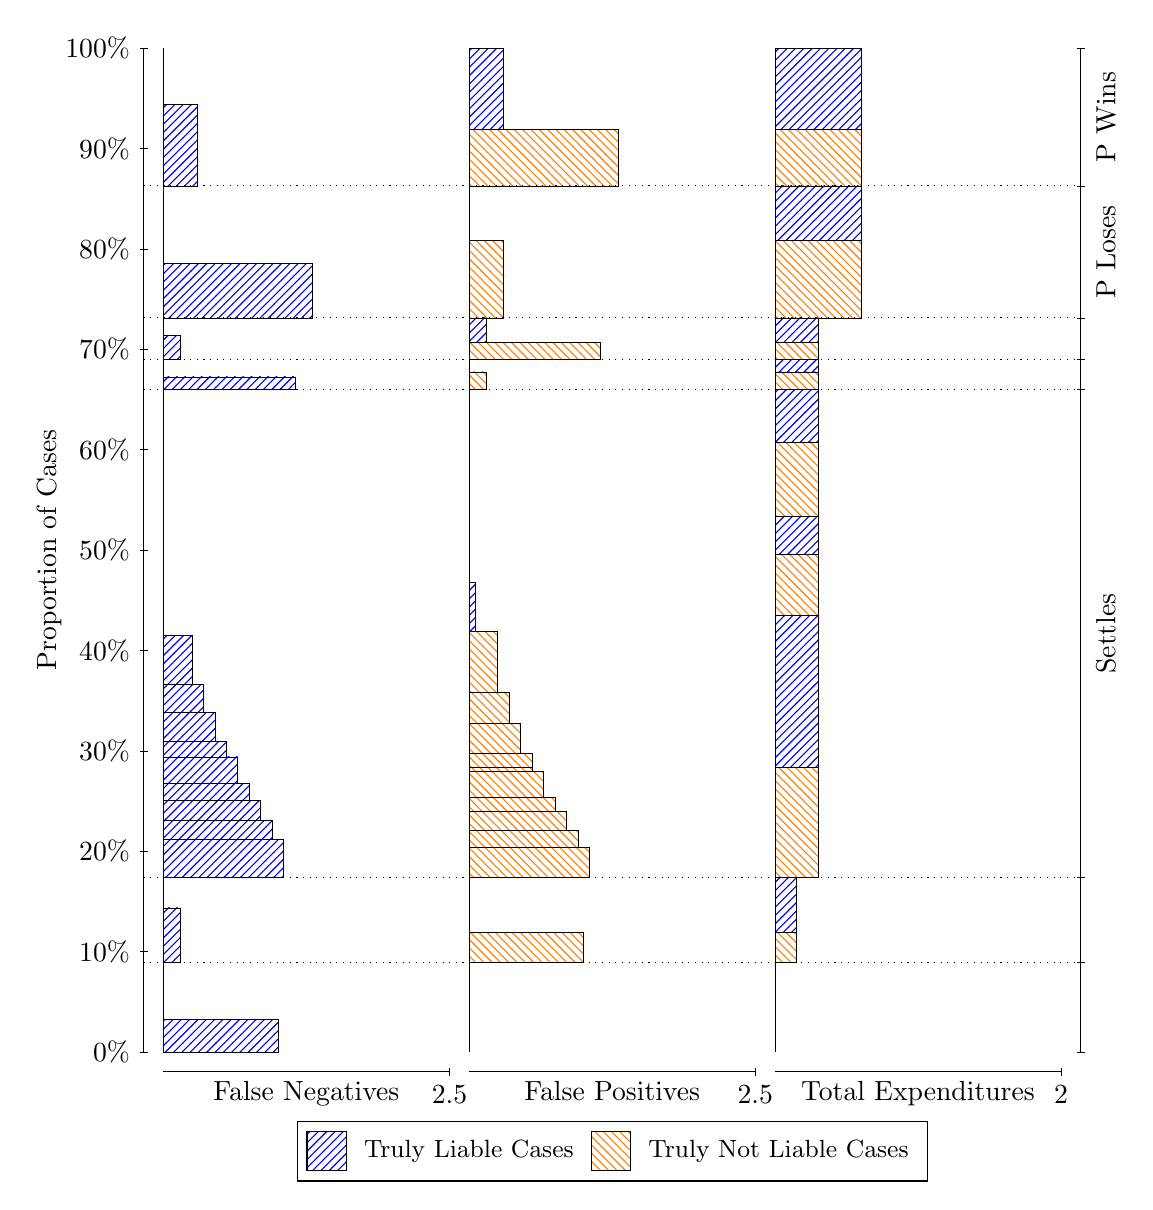
\begin{tikzpicture}
\draw[black, very thin] (1.5,1.75) -- (1.5,14.5);
\node[rotate=90, text=black, anchor=center] at (0.3, 8.125) {Proportion of Cases};
\draw[black, very thin] (1.45,1.75) -- (1.55,1.75);
\node[text=black, anchor=east] at (1.45, 1.75) {0\%};
\draw[black, very thin] (1.45,3.025) -- (1.55,3.025);
\node[text=black, anchor=east] at (1.45, 3.025) {10\%};
\draw[black, very thin] (1.45,4.3) -- (1.55,4.3);
\node[text=black, anchor=east] at (1.45, 4.3) {20\%};
\draw[black, very thin] (1.45,5.575) -- (1.55,5.575);
\node[text=black, anchor=east] at (1.45, 5.575) {30\%};
\draw[black, very thin] (1.45,6.85) -- (1.55,6.85);
\node[text=black, anchor=east] at (1.45, 6.85) {40\%};
\draw[black, very thin] (1.45,8.125) -- (1.55,8.125);
\node[text=black, anchor=east] at (1.45, 8.125) {50\%};
\draw[black, very thin] (1.45,9.4) -- (1.55,9.4);
\node[text=black, anchor=east] at (1.45, 9.4) {60\%};
\draw[black, very thin] (1.45,10.675) -- (1.55,10.675);
\node[text=black, anchor=east] at (1.45, 10.675) {70\%};
\draw[black, very thin] (1.45,11.95) -- (1.55,11.95);
\node[text=black, anchor=east] at (1.45, 11.95) {80\%};
\draw[black, very thin] (1.45,13.225) -- (1.55,13.225);
\node[text=black, anchor=east] at (1.45, 13.225) {90\%};
\draw[black, very thin] (1.45,14.5) -- (1.55,14.5);
\node[text=black, anchor=east] at (1.45, 14.5) {100\%};

\draw[black, very thin] (13.4,1.75) -- (13.4,14.5);
\draw[black, very thin] (13.35,1.75) -- (13.45,1.75);
\node[anchor=west] at (13.35, 1.75) {};
\draw[black, very thin] (13.35,2.8865) -- (13.45,2.8865);
\node[anchor=west] at (13.35, 2.8865) {};
\draw[black, very thin] (13.35,3.9654) -- (13.45,3.9654);
\node[anchor=west] at (13.35, 3.9654) {};
\draw[black, very thin] (13.35,10.163) -- (13.45,10.163);
\node[anchor=west] at (13.35, 10.163) {};
\draw[black, very thin] (13.35,10.547) -- (13.45,10.547);
\node[anchor=west] at (13.35, 10.547) {};
\draw[black, very thin] (13.35,11.074) -- (13.45,11.074);
\node[anchor=west] at (13.35, 11.074) {};
\draw[black, very thin] (13.35,12.749) -- (13.45,12.749);
\node[anchor=west] at (13.35, 12.749) {};
\draw[black, very thin] (13.35,14.5) -- (13.45,14.5);
\node[anchor=west] at (13.35, 14.5) {};

\draw[black, very thin, pattern color=blue, pattern=north east lines] (1.75,1.75) rectangle (3.2033,2.1637);
\draw[black, very thin, pattern color=orange, pattern=north west lines] (1.75,2.1637) rectangle (1.75,2.8865);
\draw[black, very thin, pattern color=blue, pattern=north east lines] (1.75,2.8865) rectangle (1.968,3.5787);
\draw[black, very thin, pattern color=orange, pattern=north west lines] (1.75,3.5787) rectangle (1.75,3.9654);
\draw[black, very thin, pattern color=blue, pattern=north east lines] (1.75,3.9654) rectangle (3.276,4.4479);
\draw[black, very thin, pattern color=blue, pattern=north east lines] (1.75,4.4479) rectangle (3.1307,4.6919);
\draw[black, very thin, pattern color=blue, pattern=north east lines] (1.75,4.6919) rectangle (2.9853,4.945);
\draw[black, very thin, pattern color=blue, pattern=north east lines] (1.75,4.945) rectangle (2.84,5.163);
\draw[black, very thin, pattern color=blue, pattern=north east lines] (1.75,5.163) rectangle (2.6947,5.4965);
\draw[black, very thin, pattern color=blue, pattern=north east lines] (1.75,5.4965) rectangle (2.5493,5.6979);
\draw[black, very thin, pattern color=blue, pattern=north east lines] (1.75,5.6979) rectangle (2.404,6.0629);
\draw[black, very thin, pattern color=blue, pattern=north east lines] (1.75,6.0629) rectangle (2.2587,6.4148);
\draw[black, very thin, pattern color=blue, pattern=north east lines] (1.75,6.4148) rectangle (2.1133,7.0394);
\draw[black, very thin, pattern color=orange, pattern=north west lines] (1.75,7.0394) rectangle (1.75,10.163);
\draw[black, very thin, pattern color=blue, pattern=north east lines] (1.75,10.163) rectangle (3.4213,10.323);
\draw[black, very thin, pattern color=orange, pattern=north west lines] (1.75,10.323) rectangle (1.75,10.547);
\draw[black, very thin, pattern color=blue, pattern=north east lines] (1.75,10.547) rectangle (1.968,10.855);
\draw[black, very thin, pattern color=orange, pattern=north west lines] (1.75,10.855) rectangle (1.75,11.074);
\draw[black, very thin, pattern color=blue, pattern=north east lines] (1.75,11.074) rectangle (3.6393,11.765);
\draw[black, very thin, pattern color=orange, pattern=north west lines] (1.75,11.765) rectangle (1.75,12.749);
\draw[black, very thin, pattern color=blue, pattern=north east lines] (1.75,12.749) rectangle (2.186,13.785);
\draw[black, very thin, pattern color=orange, pattern=north west lines] (1.75,13.785) rectangle (1.75,14.5);
\draw[black, very thin, pattern color=orange, pattern=north west lines] (5.6333,1.75) rectangle (5.6333,2.4729);
\draw[black, very thin, pattern color=blue, pattern=north east lines] (5.6333,2.4729) rectangle (5.6333,2.8865);
\draw[black, very thin, pattern color=orange, pattern=north west lines] (5.6333,2.8865) rectangle (7.0867,3.2732);
\draw[black, very thin, pattern color=blue, pattern=north east lines] (5.6333,3.2732) rectangle (5.6333,3.9654);
\draw[black, very thin, pattern color=orange, pattern=north west lines] (5.6333,3.9654) rectangle (7.1593,4.3489);
\draw[black, very thin, pattern color=orange, pattern=north west lines] (5.6333,4.3489) rectangle (7.014,4.564);
\draw[black, very thin, pattern color=orange, pattern=north west lines] (5.6333,4.564) rectangle (6.8687,4.8024);
\draw[black, very thin, pattern color=orange, pattern=north west lines] (5.6333,4.8024) rectangle (6.7233,4.9866);
\draw[black, very thin, pattern color=orange, pattern=north west lines] (5.6333,4.9866) rectangle (6.578,5.3146);
\draw[black, very thin, pattern color=orange, pattern=north west lines] (5.6333,5.3146) rectangle (6.4327,5.369);
\draw[black, very thin, pattern color=orange, pattern=north west lines] (5.6333,5.369) rectangle (6.4327,5.5461);
\draw[black, very thin, pattern color=orange, pattern=north west lines] (5.6333,5.5461) rectangle (6.2873,5.9212);
\draw[black, very thin, pattern color=orange, pattern=north west lines] (5.6333,5.9212) rectangle (6.142,6.3165);
\draw[black, very thin, pattern color=orange, pattern=north west lines] (5.6333,6.3165) rectangle (5.9967,7.089);
\draw[black, very thin, pattern color=blue, pattern=north east lines] (5.6333,7.089) rectangle (5.706,7.7137);
\draw[black, very thin, pattern color=blue, pattern=north east lines] (5.6333,7.7137) rectangle (5.6333,10.163);
\draw[black, very thin, pattern color=orange, pattern=north west lines] (5.6333,10.163) rectangle (5.8513,10.387);
\draw[black, very thin, pattern color=blue, pattern=north east lines] (5.6333,10.387) rectangle (5.6333,10.547);
\draw[black, very thin, pattern color=orange, pattern=north west lines] (5.6333,10.547) rectangle (7.3047,10.766);
\draw[black, very thin, pattern color=blue, pattern=north east lines] (5.6333,10.766) rectangle (5.8513,11.074);
\draw[black, very thin, pattern color=orange, pattern=north west lines] (5.6333,11.074) rectangle (6.0693,12.058);
\draw[black, very thin, pattern color=blue, pattern=north east lines] (5.6333,12.058) rectangle (5.6333,12.749);
\draw[black, very thin, pattern color=orange, pattern=north west lines] (5.6333,12.749) rectangle (7.5227,13.463);
\draw[black, very thin, pattern color=blue, pattern=north east lines] (5.6333,13.463) rectangle (6.0693,14.5);
\draw[black, very thin, pattern color=orange, pattern=north west lines] (9.5167,1.75) rectangle (9.5167,2.4729);
\draw[black, very thin, pattern color=blue, pattern=north east lines] (9.5167,2.4729) rectangle (9.5167,2.8865);
\draw[black, very thin, pattern color=orange, pattern=north west lines] (9.5167,2.8865) rectangle (9.7892,3.2732);
\draw[black, very thin, pattern color=blue, pattern=north east lines] (9.5167,3.2732) rectangle (9.7892,3.9654);
\draw[black, very thin, pattern color=orange, pattern=north west lines] (9.5167,3.9654) rectangle (10.062,5.369);
\draw[black, very thin, pattern color=blue, pattern=north east lines] (9.5167,5.369) rectangle (10.062,7.295);
\draw[black, very thin, pattern color=orange, pattern=north west lines] (9.5167,7.295) rectangle (10.062,8.0675);
\draw[black, very thin, pattern color=blue, pattern=north east lines] (9.5167,8.0675) rectangle (10.062,8.55);
\draw[black, very thin, pattern color=orange, pattern=north west lines] (9.5167,8.55) rectangle (10.062,9.4975);
\draw[black, very thin, pattern color=blue, pattern=north east lines] (9.5167,9.4975) rectangle (10.062,10.163);
\draw[black, very thin, pattern color=orange, pattern=north west lines] (9.5167,10.163) rectangle (10.062,10.387);
\draw[black, very thin, pattern color=blue, pattern=north east lines] (9.5167,10.387) rectangle (10.062,10.547);
\draw[black, very thin, pattern color=orange, pattern=north west lines] (9.5167,10.547) rectangle (10.062,10.766);
\draw[black, very thin, pattern color=blue, pattern=north east lines] (9.5167,10.766) rectangle (10.062,11.074);
\draw[black, very thin, pattern color=orange, pattern=north west lines] (9.5167,11.074) rectangle (10.607,12.058);
\draw[black, very thin, pattern color=blue, pattern=north east lines] (9.5167,12.058) rectangle (10.607,12.749);
\draw[black, very thin, pattern color=orange, pattern=north west lines] (9.5167,12.749) rectangle (10.607,13.463);
\draw[black, very thin, pattern color=blue, pattern=north east lines] (9.5167,13.463) rectangle (10.607,14.5);
\draw[black, dotted] (1.5,2.8865) -- (13.4,2.8865);
\draw[black, dotted] (1.5,3.9654) -- (13.4,3.9654);
\draw[black, dotted] (1.5,10.163) -- (13.4,10.163);
\draw[black, dotted] (1.5,10.547) -- (13.4,10.547);
\draw[black, dotted] (1.5,11.074) -- (13.4,11.074);
\draw[black, dotted] (1.5,12.749) -- (13.4,12.749);
\draw[black, very thin] (1.75,1.5) -- (5.3833,1.5);
\node[text=black, anchor=north] at (3.5667, 1.5) {False Negatives};
\draw[black, very thin] (5.3833,1.45) -- (5.3833,1.55);
\node[text=black, anchor=north] at (5.3833, 1.45) {2.5};

\draw[black, very thin] (5.6333,1.5) -- (9.2667,1.5);
\node[text=black, anchor=north] at (7.45, 1.5) {False Positives};
\draw[black, very thin] (9.2667,1.45) -- (9.2667,1.55);
\node[text=black, anchor=north] at (9.2667, 1.45) {2.5};

\draw[black, very thin] (9.5167,1.5) -- (13.15,1.5);
\node[text=black, anchor=north] at (11.333, 1.5) {Total Expenditures};
\draw[black, very thin] (13.15,1.45) -- (13.15,1.55);
\node[text=black, anchor=north] at (13.15, 1.45) {2};



\node[text=black, centered, rotate=90] at (13.72, 7.0642) {Settles};


\node[text=black, centered, rotate=90] at (13.72, 11.911) {P Loses};
\node[text=black, centered, rotate=90] at (13.72, 13.624) {P Wins};

\draw (7.449999999999999,1.5) node[draw=none] (baseCoordinate) {};
\begin{scope}[align=center]
        \matrix[scale=0.5, draw=black, below=0.5cm of baseCoordinate, nodes={draw}, column sep=0.1cm]{
            \node[rectangle, draw, minimum width=0.5cm, minimum height=0.5cm, pattern color=blue, pattern=north east lines] {}; &
            \node[draw=none, font=\small, text=black] (B) {Truly Liable Cases}; &
            \node[rectangle, draw, minimum width=0.5cm, minimum height=0.5cm, pattern color=orange, pattern=north west lines] {}; &
            \node[draw=none, font=\small, text=black] (B) {Truly Not Liable Cases}; \\
            };
\end{scope}

\end{tikzpicture}
\end{document}